\section{Introduction} 
\label{sec:intro}
Large language models (LLMs) are increasingly used as natural-language (NL) interfaces for querying tabular data, making Table Question Answering (Table QA) a natural testbed for evidence retrieval, numerical operations, and analytical reasoning over structured information. Most Table QA benchmarks assume that structure is \emph{explicit}, as in clean relational schemas, and that the relevant evidence is contained in a single table or connected through predefined database relations. Many real spreadsheets and reports are instead \emph{non-relational}: the structure needed to answer a question is encoded in the presentation itself, through hierarchical headers, merged cells, blank regions, unit conventions, noisy entries, or implicit dependencies within and across tables~\cite{1.10}. This is a blind spot in current Table QA evaluation; standards bodies such as the U.S. National Institute of Standards and Technology (NIST) and the World Wide Web Consortium (W3C) have highlighted tabular-data heterogeneity and the need for standardized representations to enable reliable automated analysis, underscoring that current benchmarks' focus on explicit relational schemas leaves non-relational presentations under-addressed~\cite{nist_bdif_2015,w3c_csvw_2018}. A model may answer correctly over a clean relational table yet fail on a non-relational rendering of the same evidence, especially when that evidence is distributed across multiple tables (\autoref{fig:nonrelhurts}; \S\ref{app:generating_non_rel}). Characterizing this failure mode requires controlled benchmarks that preserve the underlying evidence and gold answer across alternative renderings, while allowing systematic variation in domain, layout, perturbations, unit conventions, and cross-table evidence distribution.
\begin{figure}[t]
    \centering
    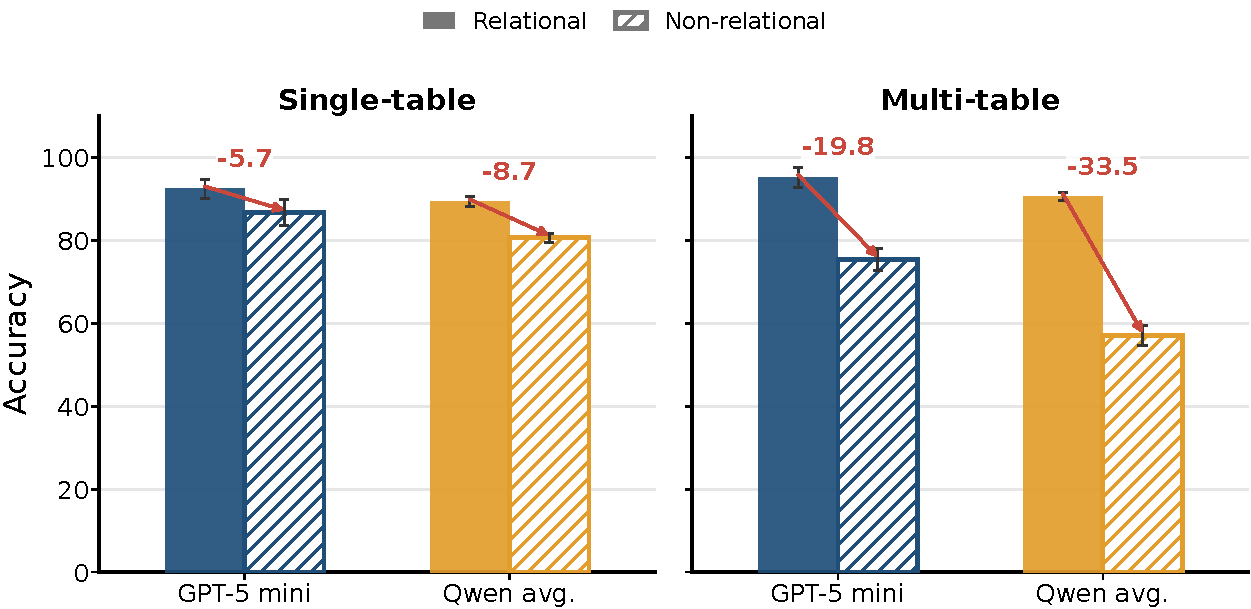
\includegraphics[width=0.48\textwidth]{img/rel_to_nonrel.pdf}
    \caption{Motivating comparison between relational and non-relational presentations: each question is evaluated on relational and non-relational variants of the same underlying data in both single- and multi-table settings. The figure reports exact-match accuracy (\%) for \texttt{gpt-5-mini} and Qwen-family models on a sample of 192 questions from Spider and Kaggle datasets.}
    \label{fig:nonrelhurts}
\end{figure}
\begin{figure*}[t]
    \centering
    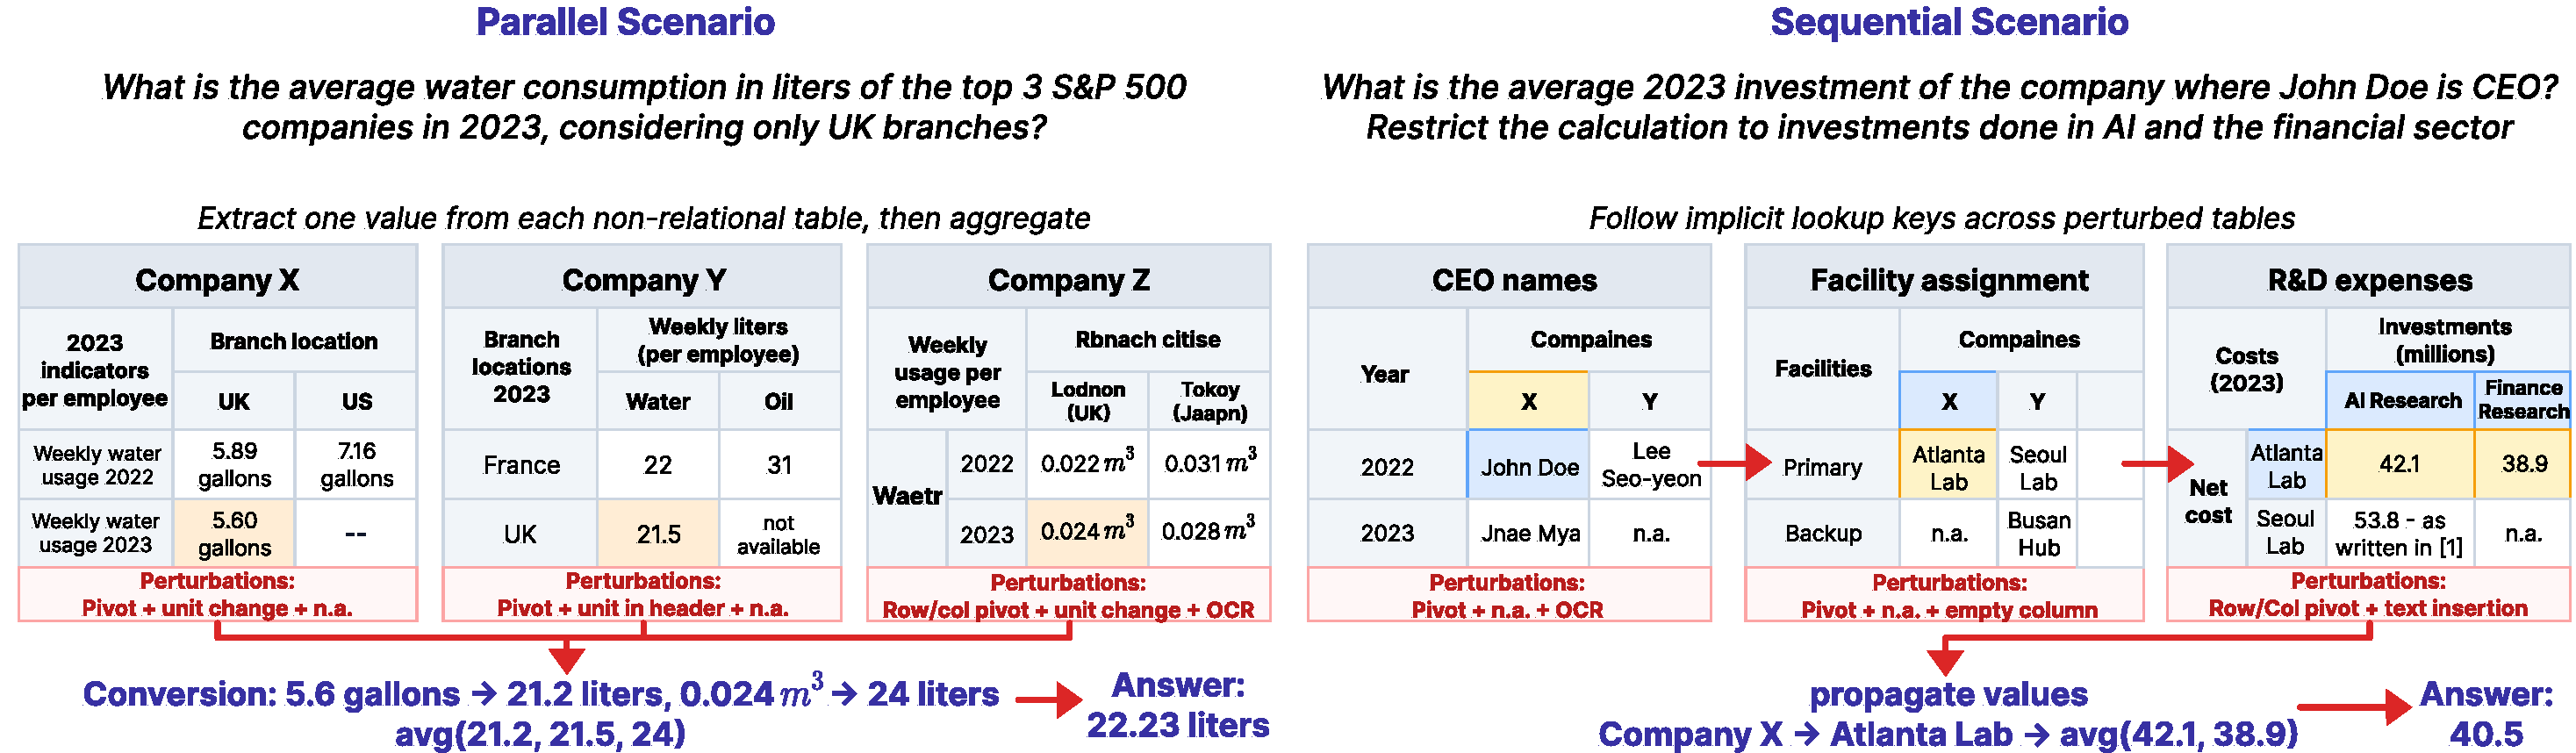
\includegraphics[width=0.99\textwidth]{img/q_types.pdf}
    \caption{Multi-table parallel and sequential scenarios generated by \name over non-relational tables. Parallel questions extract and aggregate values across perturbed tables; sequential questions propagate lookup keys across tables before aggregating final values.}
    \label{fig:questiontypes}
\end{figure*}
Existing Table QA resources address only part of this need and fall into two families. (i)~\emph{Manually curated} relational and non-relational benchmarks offer realistic tables (\S\ref{sec:rw}) but fix the domain, layout, question distribution, reasoning regime, and table count, with few targeting genuine multi-table reasoning~\cite{1.26,1.16}. Extending them means hand-crafting new tables, questions, units, missing values, perturbations, and gold answers, which is costly to scale, hard to adapt, and increasingly contaminated in recent LLMs~\cite{datacontamination}. (ii)~\emph{Automatic generation} methods are scalable and yield verifiable supervision, but operate over existing relational databases~\cite{PapicchioPC23,5.5,5.8}, which dictate what can be generated: the practitioner cannot freely set the domain, perturbations, unit conventions, or the number of tables a question spans, precisely the axes needed to probe non-relational multi-table reasoning.
To probe these axes and generate non-relational Table QA instances, one natural workaround would be to convert relational tables from existing Table QA benchmarks into non-relational views. However, post-hoc conversion falls short on two counts. (i)~\emph{Practically}, most relational tables resist dense hierarchical rendering: pivoting their attributes yields sparse layouts or missing combinations, so only a small fraction of Spider~\cite{1.6}, BIRD~\cite{1.20}, and BEAVER~\cite{1.30} tables convert into realistic dense or hierarchical views, and this constraint becomes even tighter in multi-table scenarios (\S\ref{app:generating_non_rel}). (ii)~\emph{By design}, converted data inherits the source's schema, content, and relations, granting no independent control over reasoning structure, evidence distribution, and tabular presentation. This lack of control also limits question diversity, as non-relational multi-table QA may contain two complementary evidence-flow question patterns (\autoref{fig:questiontypes}): \emph{parallel}, where values retrieved independently from different tables are aggregated, and \emph{sequential}, where intermediate lookup keys are propagated across tables. 
A non-relational Table QA generator must therefore build novel benchmarks from scratch, which is the only way to produce instances diverse in domain, perturbations, table count, and question patterns. 
We introduce \name, a from-scratch framework for generating automatically verifiable QA benchmarks over multiple non-relational tables, with explicit control over parallel and sequential evidence-flow patterns. Unlike post-hoc conversion, \name synthesizes its own latent source rather than adapting an existing database. Given a target domain and lightweight controls such as attribute cardinalities and table count, \name uses an LLM to define a domain-specific schema and instantiate a \emph{latent relational source}. From this source, it derives executable SQL programs with scalar answers, renders perturbed \emph{non-relational views}, and verbalizes the programs into NL questions. The rendering stage combines established Table QA perturbations~\cite{2.4,2.5,2.6,2.8} with pivots, hierarchical headers, merged cells, and unit conversions. This design \emph{decouples supervision from presentation}: answers are computed and verified on the latent relational source, while tested models see only the perturbed non-relational views.
\begin{table*}[t]
\centering
\fontsize{8.8pt}{10pt}\selectfont
\setlength{\tabcolsep}{1.10pt}
\renewcommand{\arraystretch}{1.15}
\begin{tabular}{llccc cccc}
\toprule
\textbf{Class} &
\textbf{Approach} &
\multicolumn{3}{c}{\textbf{Generated artifacts}} &
\multicolumn{4}{c}{\textbf{Reasoning / evaluation control}} \\
\cmidrule(lr){3-5}
\cmidrule(lr){6-9}
& & Tbl. & NLQ & Ans. & Pert. & Rel. & Non-rel. & \# tables \\
\midrule
\multirow{4}{*}{Perturbation}
& Dr.Spider~\cite{2.6}   & \xmark & \xmark & \xmark & Sch/Txt/Cell & \checkmark & \xmark & SB \\
& EvoSchema~\cite{2.8}   & \xmark & \xmark & \xmark & Sch          & \checkmark & \xmark & SB \\
& ADVETA~\cite{2.5}      & \xmark & \xmark & \xmark & Sch          & \checkmark & \xmark & SB \\
& FREB-TQA~\cite{2.9}    & \xmark & \xmark & \xmark & Cell/Lay     & \xmark     & \checkmark & 1 \\
\midrule
\multirow{3}{*}{\makecell[l]{Tabular\\synthesis}}
& REaLTabFormer~\cite{5.9} & \checkmark & \xmark & \xmark & \xmark & \checkmark & \xmark & N/A \\
& GOGGLE~\cite{5.10}       & \checkmark & \xmark & \xmark & \xmark & \checkmark & \xmark & N/A \\
& TabGen-ICL~\cite{5.1}    & \checkmark & \xmark & \xmark & \xmark & \checkmark & \xmark & N/A \\
\midrule
\multirow{8}{*}{\makecell[l]{QA / SQL\\synthesis}}
& \citet{9.1}           & \xmark     & \xmark     & \checkmark & \xmark & \checkmark & \xmark & 1 \\
& \citet{9.2}           & \xmark     & \checkmark & \checkmark & \xmark & \checkmark & \xmark & 1 \\
& \citet{9.5}           & \xmark     & \xmark     & \checkmark & \xmark & \checkmark & \xmark & SB \\
& ER-Bench~\cite{5.5}   & \xmark     & \checkmark & \checkmark & \xmark & \checkmark & \xmark & SB \\
& SPARTA~\cite{5.8}     & \xmark     & \checkmark & \checkmark & \xmark & \checkmark & \xmark & SB \\
& DSQG-Syn~\cite{9.8}   & \xmark     & \checkmark & \checkmark & \xmark & \checkmark & \xmark & SB \\
& SQLForge~\cite{9.7}   & \checkmark & \checkmark & \checkmark & \xmark & \checkmark & \xmark & SB \\
& SYNQL~\cite{9.6}      & \xmark     & \checkmark & \checkmark & \xmark & \checkmark & \xmark & SB \\
\midrule
\textbf{Ours}
& \textbf{\name}
& \checkmark
& \checkmark
& \checkmark
& \textbf{Sch/Cell/Lay/Num}
& \checkmark
& \checkmark
& \textbf{GC} \\
\bottomrule
\end{tabular}
\caption{
Comparison with data-generation approaches.
Tbl., NLQ, and Ans. denote generated tables, natural-language questions, and automatically verifiable answers.
Perturbations are abbreviated as schema/name (Sch), text/query (Txt), cell/content (Cell), layout/structure (Lay), and numerical/unit (Num).
The number of tables is either fixed to one, source-bounded (SB), or generator-controlled (GC). 
}
\label{tab:related_work_comparison}
\end{table*}
We evaluate \name on financial and environmental scenarios with up to 20 parallel and 5 sequentially connected tables per question, using \texttt{gpt-5-mini} and Qwen-family models. As table count increases, accuracy drops by up to 39.6 points in parallel settings and 32.5 points in sequential settings, while unit heterogeneity causes additional losses of up to 50.1 points, with strong domain dependence. The drop generalizes to real tables: on the few real tables admitting non-relational rendering, perturbation costs 7.95 points single-table and 30.05 multi-table (\S\ref{app:generating_non_rel}). 
Manual inspection finds 95.9\% of 240 generated questions correct. 
Finally, \name-generated data complements scarce in-domain supervision, as combining \name with the small GRI-QA~\cite{1.16} training set yields the best results on the GRI-QA test set.
In summary, our contributions are:
(i) we introduce \name, a from-scratch generator of automatically verifiable numerical QA over multiple non-relational tables;
(ii) we define controllable parallel and sequential evidence-flow patterns with answer-preserving structural, cell-level, and unit-based perturbations;
(iii) we show that table count, non-relational presentation, and unit heterogeneity substantially degrade LLM performance, and confirm on perturbed real tables that non-relationality is especially harmful in multi-table settings;
(iv) we validate generated-question correctness and show that \name-generated data provides effective supervision that complements scarce in-domain data;
(v) we release code and generated datasets\footnote{\href{https://anonymous.4open.science/r/Gradino-DBF6/}{Anonymous Github link}}. 
